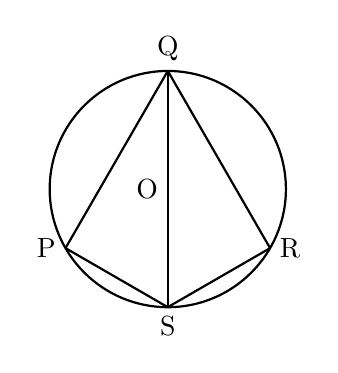
\begin{tikzpicture}[scale=1]

  % Define the center of the circle
  \coordinate (O) at (0,0);

  % Define the radius of the circle
  \def\R{1.5}

  % Draw the circle
  \draw[thick] (O) circle (\R);

  % Define the points on the circle
  % Approximate the angles to match the image
  % Q is at the top
  \coordinate (Q) at (90:\R);
  % S is at the bottom
  \coordinate (S) at (270:\R);
  % P is on the left
  \coordinate (P) at (210:\R);
  % R is on the right
  \coordinate (R) at (330:\R);

  % Draw the lines forming the cyclic quadrilateral PQRS
  \draw[thick] (P) -- (Q);
  \draw[thick] (Q) -- (R);
  \draw[thick] (R) -- (S);
  \draw[thick] (S) -- (P);

  % Draw the line segment QS
  \draw[thick] (Q) -- (S);

  % Add labels for the points
  \node[above] at (Q) {Q};
  \node[below] at (S) {S};
  \node[left] at (P) {P};
  \node[right] at (R) {R};

  % Add the label 'O' near the center (slightly to the left as in the image)
  \node[left] at (0, 0) {O};

\end{tikzpicture}